\documentclass{article}%
\usepackage[T1]{fontenc}%
\usepackage[utf8]{inputenc}%
\usepackage{lmodern}%
\usepackage{textcomp}%
\usepackage{lastpage}%
\usepackage{authblk}%
\usepackage{graphicx}%
%
\title{The phosphatidylinositol{-}3 kinase I inhibitor BKM120 induces cell death in B{-}chronic lymphocytic leukemia cells in vitro}%
\author{Jason Hunt}%
\affil{Department of Surgery, Gastroenterological Surgery, Graduate School of Medicine, Osaka University, Suita, Osaka, Japan}%
\date{01{-}01{-}2013}%
%
\begin{document}%
\normalsize%
\maketitle%
\section{Abstract}%
\label{sec:Abstract}%
SAN DIEGO {-} A mouse mutation identified in a series of genetic studies may offer clues about new targets for therapies to treat disorders including diabetes and heart disease.\newline%
The study, published in the current online issue of the American Journal of Human Genetics, tracked the genes of mice bred with the mutation in four separate experiments: the A common race, the A{-}73 subgroup in mice, the A defect in mice bred with multiple A mutations, and the C gene in mice bred with just one A mutation. All of the mice had less blood supply to their blood vessels, but the differences werent statistically significant.\newline%
The study used RNA sequencing to identify the 25 genes that were deleted from the mices genomes after they underwent the one{-}shot treatment. Existing therapies usually work by killing the mutated gene at the molecular level, which makes eliminating the defective gene easier but also takes longer to work at the cellular level. In this treatment, protein fragments within the mouses blood stream become involved in maintaining a vital chemical regulator, a white blood cell

%
\subsection{Image Analysis}%
\label{subsec:ImageAnalysis}%


\begin{figure}[h!]%
\centering%
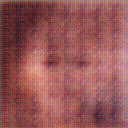
\includegraphics[width=150px]{500_fake_images/samples_5_130.png}%
\caption{A Black And White Photo Of A Black And White Striped Tie}%
\end{figure}

%
\end{document}